

\documentclass[12pt]{report}
\usepackage[utf8]{inputenc}
\usepackage[russian]{babel}
\usepackage[14pt]{extsizes}
\usepackage{listings}
\usepackage{graphicx}
\usepackage{amsmath,amsfonts,amssymb,amsthm,mathtools} 
\usepackage{pgfplots}
\usepackage{filecontents}
\usepackage{float}
\usepackage{indentfirst}
\usepackage{eucal}
\usepackage{enumitem}
%s\documentclass[openany]{book}
\frenchspacing

\usepackage{titlesec}
\titleformat{\section}
{\normalsize\bfseries}
{\thesection}
{1em}{}
\titlespacing*{\chapter}{0pt}{-30pt}{8pt}
\titlespacing*{\section}{\parindent}{*4}{*4}
\titlespacing*{\subsection}{\parindent}{*4}{*4}

\usepackage{indentfirst} % Красная строка

\usetikzlibrary{datavisualization}
\usetikzlibrary{datavisualization.formats.functions}

\usepackage{amsmath}

\usepackage{amssymb}

% Для листинга кода:
\lstset{ %
	language=lisp,                 % выбор языка для подсветки (здесь это С)
	texcl=true,
	extendedchars=\true,
	basicstyle=\small\sffamily, % размер и начертание шрифта для подсветки кода
	numbers=left,               % где поставить нумерацию строк (слева\справа)
	numberstyle=\tiny,           % размер шрифта для номеров строк
	stepnumber=1,                   % размер шага между двумя номерами строк
	numbersep=5pt,                % как далеко отстоят номера строк от подсвечиваемого кода
	showspaces=false,            % показывать или нет пробелы специальными отступами
	showstringspaces=false,      % показывать или нет пробелы в строках
	showtabs=false,             % показывать или нет табуляцию в строках
	frame=single,              % рисовать рамку вокруг кода
	tabsize=2,                 % размер табуляции по умолчанию равен 2 пробелам
	captionpos=t,              % позиция заголовка вверху [t] или внизу [b] 
	breaklines=true,           % автоматически переносить строки (да\нет)
	breakatwhitespace=false, % переносить строки только если есть пробел
	escapeinside={\#*}{*)},  % если нужно добавить комментарии в коде
	%inputencoding=utf8x,
	%extendedchars=\true
}



\usepackage[left=2cm,right=2cm, top=2cm,bottom=2cm,bindingoffset=0cm]{geometry}
% Для измененных титулов глав:
\usepackage{titlesec, blindtext, color} % подключаем нужные пакеты
\definecolor{gray75}{gray}{0.75} % определяем цвет
\newcommand{\hsp}{\hspace{20pt}} % длина линии в 20pt
% titleformat определяет стиль
\titleformat{\chapter}[hang]{\Huge\bfseries}{\thechapter\hsp\textcolor{gray75}{|}\hsp}{0pt}{\Huge\bfseries}


% plot
\usepackage{pgfplots}
\usepackage{filecontents}
\usetikzlibrary{datavisualization}
\usetikzlibrary{datavisualization.formats.functions}

\begin{document}
	%\def\chaptername{} % убирает "Глава"
	\thispagestyle{empty}
	\begin{titlepage}
		\noindent \begin{minipage}{0.15\textwidth}
			
\includegraphics[width=\linewidth]{img/b_logo}
		\end{minipage}
		\noindent\begin{minipage}{0.9\textwidth}\centering
			\textbf{Министерство науки и высшего образования Российской Федерации}\\
			\textbf{Федеральное государственное бюджетное образовательное учреждение высшего образования}\\
			\textbf{~~~«Московский государственный технический университет имени Н.Э.~Баумана}\\
			\textbf{(национальный исследовательский университет)»}\\
			\textbf{(МГТУ им. Н.Э.~Баумана)}
		\end{minipage}
		
		\noindent\rule{18cm}{3pt}
		\newline\newline
		\noindent ФАКУЛЬТЕТ $\underline{\text{«Информатика и системы управления»}}$ \newline\newline
		\noindent КАФЕДРА $\underline{\text{«Программное обеспечение ЭВМ и информационные технологии»}}$\newline\newline\newline\newline\newline
		
		\begin{center}
			\noindent\begin{minipage}{1.1\textwidth}\centering
				\Large\textbf{  Отчет по лабораторной работе №4}\newline
				\textbf{по дисциплине <<Функциональное и логическое}\newline
				\textbf{~~~программирование>>}\newline\newline
			\end{minipage}
		\end{center}
		
		\noindent\textbf{Тема} $\underline{\text{Использование управляющих структур, работа со списками}}$\newline\newline
		\noindent\textbf{Студент} $\underline{\text{Зайцева А. А.~~~~~~~~~~~~~~~~~~~~~~~~~~~~~~~~~~~~~~~~~~}}$\newline\newline
		\noindent\textbf{Группа} $\underline{\text{ИУ7-62Б~~~~~~~~~~~~~~~~~~~~~~~~~~~~~~~~~~~~~~~~~~~~~~~~~~}}$\newline\newline
		\noindent\textbf{Оценка (баллы)} $\underline{\text{~~~~~~~~~~~~~~~~~~~~~~~~~~~~~~~~~~~~~~~~~~~~~~~~~}}$\newline\newline
		\noindent\textbf{Преподаватели} $\underline{\text{Толпинская Н.Б., Строганов Ю. В.~~~~~~~~~~~~~~~~~~~~~~~~~~~~}}$\newline\newline\newline
		
		\begin{center}
			\vfill
			Москва~---~\the\year
			~г.
		\end{center}
	\end{titlepage}
	
\chapter*{Теоретические вопросы}

\section*{1. Синтаксическая форма и хранение программы в памяти}

Программа на Lisp представляет собой вызов функции на верхнем уровне. Все операции над данными оформляются и  записываются как функции, которые имеют значение, даже если их основное предназначение – осуществление некоторого побочного эффекта. Программа является ничем иным, как набором запрограммированных функций.

\textbf{Синтаксически} программа оформляется в виде S-выражения (обычно -- списка -- частного случая точечной пары), которое очень часто может быть структурированным. Наличие скобок является признаком структуры. 

По определению:
\begin{itemize}
	\item S-выражение ::= <атом> | <точечная пара>

	\item Атомы:
\begin{itemize} 
	\item символы (идентификаторы) – синтаксически – набор литер (букв и цифр), начинающихся с буквы;
	\item специальные символы – {T, Nil} (используются для обозначения логических констант);
	\item самоопределимые атомы – натуральные числа, дробные числа, вещественные числа, строки – последовательность символов, заключенных в двойные апострофы (например, “abc”);
\end{itemize} 


\item Точечная пара ::= (<атом> . <атом>) | (<атом> . <точечная пара>) | (<точечная пара> . <атом>) | (<точечная пара> . <точечная пара>);

\item Список ::= <пустой список> | <непустой список>, где 

<пустой список> ::= () | Nil,

<непустой список> ::= (<первый элемент> . <хвост>),

<первый элемент> ::= <S-выражение>,

<хвост> ::= <список>.

\end{itemize}

Атомы представляются \textbf{в памяти} пятью указателями  (name, value, function, property, package), а любая непустая структура --  списковой ячейкой (бинарным узлом), хранящей два указателя: на голову (первый элемент) и хвост -- все остальное.











\section*{2. Трактовка элементов списка.}

По определению списка, приведенному выше: если список непустой, то он представляет из себя точечную пару из  <первого элемента> и <хвоста>, где <первый элемент> -- это <S-выражение>, а <хвост> -- это <список>.

Список можно вычислить, если он представляет собой обращение к  функции, или функциональный вызов: (f e1 e2 … en), где f – символьный атом, имя вызываемой функции; e1, e2, …, en – аргументы этой функции; n - число аргументов функции.

В случае n=0 имеем вызов функции без аргументов: (f). Обычно e1, e2, …, en являются вычислимыми выражениями и вычисляются последовательно слева направо.

Таким образом, если в процессе работы лисп-интерпретатора  требуется вычислить некоторый список, то первым элементом этого   списка должно быть имя функции. Если это не так, лисп-интерпретатор  сообщает об ошибке и прерывает вычисление текущего выражения  программы.


\section*{3. Порядок реализации программы.}

Типичная лисп-программа включает:
\begin{itemize}
	\item определения новых функций на базе встроенных функций и других функций, определённых в этой программе;
	\item {вызовы этих новых функций для конкретных значений их аргументов.}
\end{itemize}

Как отмечалось выше, программа на Lisp представляет собой вызов функции на верхнем уровне и синтаксически оформляется в виде S-выражения. Вычисление программы реализует лисп-интерпретатор, который считывает очередную входящую в программу форму, вычисляет её (анализирует функцией eval) и выводит полученный результат (S-выражение).

Eval выполняет двойное  вычисление своего аргумента. Эта функция является обычной, и первое  вычисление аргумента выполняет так же, как и любая обычная функция.  Полученное при этом выражение вычисляется ещё раз. Такое двойное  вычисление может понадобиться либо для снятия блокировки вычислений (установленной функцией quote), либо же для вычисления сформированного в ходе первого вычисления нового функционального вызова.

\clearpage
Вызов (eval S-выражение):

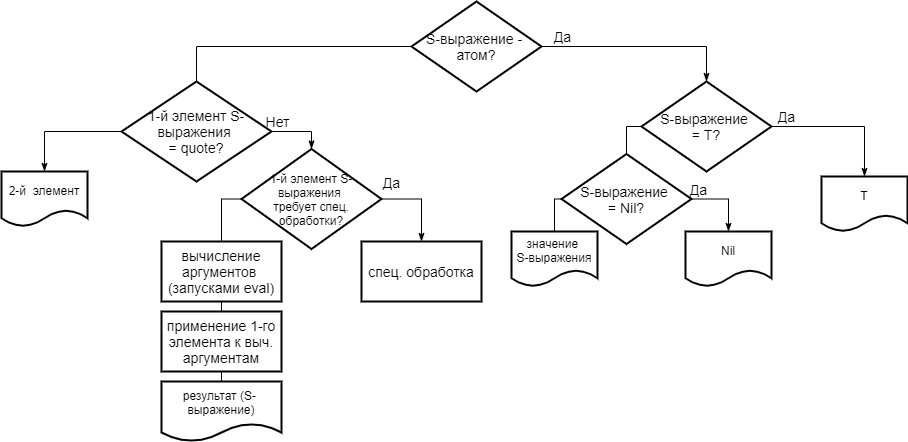
\includegraphics[scale=0.5]{img/eval}

\section*{4. Способы определения функции}

Функцией называется правило, по которому каждому значению одного или нескольких  аргументов ставится в соответствие конкретное значение результата. 


Функционалом, или функцией высшего порядка называется функция, аргументом или  результатом которой является другая функция.

Форма -- функция, которая особым образом обрабатывает свои аргументы, т. е. требует специальной обработки.


Определение функций пользователя в Lisp-е возможно двумя способами.


\begin{itemize}
	\item Базисный способ  определения  функции - использование $\lambda$-выражения ($\lambda$-нотации). Так создаются функции без имени.
	
	$\lambda$-выражение: (lambda $\lambda$-список форма), 
	где $\lambda$-список --  это формальные параметры функции (список аргументов), а форма -- это тело функции.
	
	Вызов такой функции осуществляется следующим способом: ($\lambda$-выражение последовательность\_форм), 
	где последовательность\_форм -- это фактические параметры.
	
	Вычисление функций без имени может быть также выполнено с использованием функционала apply: (apply $\lambda$-выражение последовательность\_форм), где последовательность\_форм -- это список фактических параметров; или с использованием функционала funcall: (funcall $\lambda$-выражение последовательность\_форм), где последовательность\_форм -- это фактические параметры.
	
	Функционал apply является обычной функцией с двумя  вычисляемыми аргументами, обращение к ней имеет вид: (apply F L), где F – функциональный аргумент и L -- список, рассматриваемый как список фактических параметров для F. Значение функционала -- результат применения F к этим фактическим параметрам.
	
	Функционал funcall – особая функция с вычисляемыми аргументами, обращение к ней: (funcall F e1 … en), n $\geqslant 0$. Её   действие аналогично apply, отличие состоит в том, что аргументы  применяемой функции F задаются не списком, а по отдельности. 
	
	funcall используется тогда, когда во время написания кода количество аргументов известно, apply -- когда неизвестно.
	
	\item Другой способ определения функции -- использование макро-определения defun: 
	
	(defun имя\_функции $\lambda$-выражение), 
	
	или  в облегченной форме:
	
	(defun имя\_функции $(x_1, x_2, ..., x_k)$ форма), 
	где $(x_1, x_2, ..., x_k)$ -- это  список аргументов.
	
	В качестве имени функции выступает символьный атом. 
	Вызов именованной функции осуществляется следующим образом: (имя\_функции последовательность\_форм), 
	где последовательность\_форм -- это фактические параметры.
	Также для ее вызова можно воспользоваться рассмотренными выше функционалами funcall (например, (foo 1 2 3) === (funcall \#'foo 1 2 3)) и apply (например, (apply \#'plot plot-data), где plot-data - список, хранящий аргументы).
	
\end{itemize}

$\lambda$-определение более эффективно, особенно при повторных вычислениях. 

Параметры функции, переданные при вызове, будут связаны с переменными в списке параметров из объявления функции. Еще один способ связывания формальных параметров с фактическими -- использование функции let:

(let ((x1 p1) (x2 p2) ... (xk pk))  e),

где xi -- формальные параметры, pi -- фактические параметры (могут быть формами), e -- форма (что делать).

\clearpage
\section*{Из указаний к выполнению работы}

\textbf{cond}

Общий вид условного выражения:

$(cond \; (p_1  \; e_{11}  \;  e_{12}  \;  …  \;  e_{1m_1})  \;  (p_2  \;  e_{21} \;  e_{22}  \;  …  \;  e_{2m_2})  \;  …  \;  (p_n  \; e_{n1} \;  e_{n2} \;  …  \; e_{nm_n})), m_i \geqslant 0 , n \geqslant 1$

Вычисление условного выражения общего вида выполняется по  следующим правилам:

\begin{enumerate}
	\item последовательно вычисляются условия $p_1, p_2, … p_n$ ветвей выражения до тех пор, пока не встретится выражение $p_i$, значение   которого отлично от NIL;
	\item последовательно вычисляются выражения-формы $e_{i1} \;  e_{i2} \;  … \;  e_{im_i}$ соответствующей ветви, и значение последнего выражения $e_{im_i}$ возвращается в качестве значения функции cond;
	\item если все условия $p_i$ имеют значение NIL, то значением условного выражения становится NIL.
\end{enumerate}

Ветвь условного выражения может иметь вид ($p_i$), когда $m_i$ = 0. Тогда если значение pi $\neq$ NIL, значением условного выражения cond становится значение pi.

В случае, когда pi $\neq$ NIL и $m_i$ $\geqslant$ 2, то есть ветвь cond содержит более  одного выражения $e_i$, эти выражения вычисляются последовательно, и  результатом cond служит значение последнего из них $e_{im_i}$. Таким  образом, в дальнейших вычислениях может быть использовано только значение последнего выражения, и при строго функциональном  программировании случай $m_i$ $\geqslant$ 2 обычно не возникает, т.к. значения  предшествующих $e_{im_i}$ выражений пропадают. 


 
\textbf{if}

Макрофункция (If C E1 E2), встроенная в MuLisp и Common Lisp, вычисляет значение выражения E1, если значение выражения C отлично от NIL, в ином случае она вычисляет значение E2:

(defmacro If (C E1 E2) (list 'cond (list C E1) (list T E2)))

Этот макрос строит и вычисляет условное выражение cond, в котором в качестве условия первой ветви берётся выражение С (первый аргумент If), а выражения E1 и E2 (второй и третий аргумент If) размещаются соответственно на первой и второй ветви cond.


\textbf{and/or/not}

К логическим функциям-предикатам относят логическое отрицание not, конъюнкцию and и дизъюнкцию or. Первая из этих функций является обычной, а другие две – особыми, поскольку допускают произвольное количество аргументов, которые не всегда вычисляются. 

Логическое отрицание not вырабатывает соответственно: (not NIL) => T и (not T) => NIL, и может быть определено функцией (defun not (x) (eq x NIL)).


Вызов функции and, реализующей конъюнкцию, имеет вид (and e1 e2 … en), n $\geqslant$ 0. 

При вычислении этого функционального обращения последовательно слева направо вычисляются аргументы функции ei – до тех пор, пока не  встретится значение, равное NIL. В этом случае вычисление прерывается и значение функции равно NIL. Если же были вычислены все значения ei и  оказалось, что все они отличны от NIL, то результирующим значением функции and будет значение последнего выражения en .

Вызов функции-дизъюнкции имеет вид (or e1 e2 … en), n $\geqslant$ 0. 

При выполнении вызова последовательно вычисляются аргументы ei (слева направо) – до тех пор, пока не встретится значение ei, отличное от NIL. В этом случае вычисление прерывается и значение функции равно значению этого ei. Если же вычислены значения всех аргументов ei, и оказалось, что они равны NIL, то результирующее значение функции равно NIL.

При n=0 значения функций: (and)=>T, (or)=>NIL.

Таким образом, значение функции and и or не обязательно равно Т или NIL, а может быть произвольным атомом или списочным выражением.


\textbf{remove} принимает 2 аргумента и возвращает список, заданный вторым аргументом, из которого удалены все вхождения значения первого аргумента.

\textbf{sabstitute} принимает 3 аргумента и возвращает список, заданный третьим аргументом, в котором все вхождения значения второго аргумента заменены на значение первого аргумента.

Остальные функции будут рассмотрены по ходу выполнения работы.



	
\chapter*{Практические задания}	

\section*{1. Чем принципиально отличаются функции cons, list, append?}

cons принимает 2 указателя на любые S-выражения и возвращает новую cons-ячейку (списковую ячейку), содержащую 2 значения. Если второе значение не NIL и не другая cons-ячейка, то ячейка печатается как два значения в скобках, разделённые точкой (так называемая точечная пара). Иначе, по сути, эта функция включает значение первого аргумента в начало списка, являющегося значением второго аргумента. 

Функция list, составляющая список из значений своих аргументов (у которого голова -- это первый аргумент, хвост -- все остальные аргументы), создает столько списковых ячеек, сколько аргументов ей было передано. Эта функция относится к особым, поскольку у неё может быть произвольное число аргументов, но при этом все аргументы вычисляются.

append принимает произвольное количество аргументов-списков и соединяет (сливает)  элементы верхнего уровня всех списков в один список. Действие append иногда называют конкатенацией списков. В результате должен быть построен новый список.

Например: (append (list 1 2) (list 3 4)) ==> (1 2 3 4). 

С точки зрения функционального подхода, задача функции append - вернуть список (1 2 3 4) не изменяя ни одну из cons-ячеек в списках-аргументах (1 2) и (3 4). append на самом деле создаёт только две новые cons-ячейки, чтобы хранить значения 1 и 2, соединяя их вместе и делая ссылку из CDR второй ячейки на первый элемент последнего аргумента - списка (3 4). После этого функция возвращает cons-ячейку содержащую 1. Ни одна из входных cons-ячеек не была изменена, и результатом, как и требовалось, является список (1 2 3 4). Единственная хитрость в том, что результат, возвращаемый функцией append имеет общие cons-ячейки со списком (3 4). Таким образом, если последний переданный список будет модифицирован, то  итоговый список будет также изменен.


Итак, отличия: cons является базисной, list и append -- нет; list и append принимают произвольное количество аргументов (причем аргументами append могут быть только списки), cons -- фиксированное (два); cons создает точечную пару или список (в зависимости от второго аргумента), list и append -- список; cons и list создают новые списковые ячейки (все), а append имеет общие списковые ячейки с последним списком.

list и append определяются с помощью cons.

\clearpage
\textbf{Пусть (setf lst1 '( a b)); (setf lst2 '(c d))\\
	Каковы результаты вычисления следующих выражений?}

%(defvar lst1)
%(defvar lst2)
%(defvar result_cons)
%(defvar result_list)
%(defvar result_append)
%(setf lst1 '(a b))
%(setf lst2 '(c d))
%(setf result_cons (cons lst1 lst2))
%(setf result_list (list lst1 lst2))
%(setf result_append (append lst1 lst2))

\begin{lstlisting}[language=Lisp]	
	(cons lst1 lst2) => ((A B) C D)
	(list lst1 lst2) => ((A B) (C D))
	(append lst1 lst2) => (A B C D)
\end{lstlisting}


\section*{2. Каковы результаты вычисления следующих выражений, и почему?
}

\textbf{reverse} переворачивает свой список-аргумент, т.е. меняет порядок его элементов  верхнего уровня на противоположный, например:  (reverse '(A (B D) C)) => (C (B D) A). reverse является примером рекурсии, определение может быть следующим \cite{bolshakova}:

\begin{lstlisting}[language=Lisp]	
	(defun Reverse (L) 
		(cond ((null L) NIL)
			(T (append (Reverse (cdr L)) 
				 (cons (car L) NIL) )) ))
\end{lstlisting}

В этом определении реализована следующая идея рекурсивного построения требуемого списка: он получается из перевернутого хвоста исходного списка присоединением к нему справа первого элемента. 

%Для присоединения используется функция append, а не cons, т.к. последняя может добавлять элементы только в начало списка. Поскольку оба  аргумента append должны быть списками, в качестве второго аргумента берётся одноэлементный список из первого элемента исходного списка.


\textbf{last} возвращает последнюю cons-ячейку в списке. Если вызывается с целочисленным аргументом n, возвращает n ячеек (то есть по умолчанию n=1).
Если n больше или равно количеству cons-ячеек в списке, результатом будет исходный список.

%(last ()); по умолчанию n = 1 > (length ()) = 0, поэтому результатом будет исходный пустой список

\begin{lstlisting}[language=Lisp]
	; первая ветвь cond из определения reverse
	(reverse ()) => Nil 
	; передан пустой список (то есть список длины 0), а n=1  по умолчанию. 
	; 0 < 1 => результатом будет исходный список
	(last ()) => Nil 
	; при первом вызове reverse по второй ветви cond произойдет слияние: 
	; - результата вызова reverse для хвоста исходного списка (пустого списка);
	; - списка из первого элемента исходного списка (списка (а)).
	(reverse '(a)) => (A)
	; по умолчанию n=1, поэтому результат - список из одной последней ячейки 
	; исходного списка (то есть список из сисвольного атома а)
	(last '(a)) => (A)
	; для следующих двух вызовов объяснения аналогичны приведенным двум выше 
	; с учетом того, что reverse и last работают с элементами верхнего уровня
	(reverse '((a b c))) => ((A B C))
	(last '((a b c))) => ((A B C))
\end{lstlisting}

\clearpage

\section*{3. Написать, по крайней мере, два варианта функции, которая возвращает последний элемент своего списка-аргумента.}


Первый элемент перевернутого списка:
\begin{lstlisting}[language=Lisp]
	(defun f3_reverse (lst) (
		car (reverse lst)
	))
	
	(f3_reverse '(1 2 (3 4)) => (3 4))
\end{lstlisting}

Рекурсивно:
\begin{lstlisting}[language=Lisp]
	(defun f3_recursive (lst) (
		if (null (cdr lst)) 
			(car lst) 	
			(f3_recursive (cdr lst))
	))
	
	(f3_recursive '(1 2 (3 4))) => (3 4)
\end{lstlisting}



\section*{4. Написать, по крайней мере, два варианта функции, которая возвращает свой список-аргумент без последнего элемента.}


Перевернутый хвост перевернутого списка:
\begin{lstlisting}[language=Lisp]
	(defun f4_reverse (lst) (
		reverse (cdr (reverse lst))
	))
	
	(f4_reverse '((0 1) 2 (3 4))) => ((0 1) 2)
\end{lstlisting}

Рекурсивно:
\begin{lstlisting}[language=Lisp]
	(defun f4_recursive (lst) (
		if (null (cdr lst)) 
			Nil 
			(cons (car lst) (f4_recursive (cdr lst)))
	))
	
	(f4_recursive '((0 1) 2 (3 4))) => ((0 1) 2)
\end{lstlisting}

\clearpage
\section*{5. Написать простой вариант игры в кости, в котором бросаются две правильные кости.}

Если сумма выпавших очков равна 7 или 11 -- выигрыш, если выпало (1,1) или (6,6) -- игрок получает право снова бросить кости, во всех остальных случаях ход переходит ко второму игроку, но запоминается сумма выпавших очков. Если второй игрок не выигрывает абсолютно, то выигрывает тот игрок, у которого больше очков. Результат игры и значения выпавших костей выводить на экран с помощью функции print.

(символ апостроф, написанный перед словом на русском языке, ошибочно переносится после этого слова)

\begin{lstlisting}[language=Lisp]
(defun roll_dice () (+ (random 6) 1))

(defun check_continue_game (result) (
	not (or (= result 7) (= result 11)))
)

(defun make_a_move (player_i) 
	(let ((dice1 (roll_dice)) (dice2 (roll_dice)))
		(if (and (print (list 'Игрок player_i 'бросает 'кости)) (= dice1 dice2) (or (= dice1 1) (= dice1 6)))
			(and 
				(print (list 'Выпало  dice1 dice2  'Повторный 'бросок)) 
				(make_a_move player_i)
			)
			(and 
				(print (list 'Выпало dice1 dice2))
				(+ dice1 dice2)
			)
		)
	)
)
(defun compare_results (res1 res2) 
	(if (check_continue_game res2)
	  (and
		  (print (list 'Сравнение 'по 'очкам))
		  (print (list 'Игрок 1 'набрал res1))
		  (print (list 'Игрок 2 'набрал res2))
		  (cond 
			((< res1 res2) (and (print (list 'Игрок 2 'выиграл 'по 'очкам)) 2))
			((> res1 res2) (and (print (list 'Игрок 1 'выиграл 'по 'очкам)) 1))
			((and (print '(Ничья)) 0))
		  )
	  )	
	  (and (print (list 'Игрок 2 'набрал res2 'очков 'и 'выиграл 'абсолютно)) 2)
	)
)

(defun play_game () 
	(let ((res1 (make_a_move 1)))
		(if (check_continue_game res1)
			(compare_results res1 (make_a_move 2))
			(and (print (list 'Игрок 1 'набрал res1 'очков 'и 'выиграл 'абсолютно)) 1)
		)
	)
)

\end{lstlisting}

	\bibliographystyle{utf8gost705u}  % стилевой файл для оформления по ГОСТу
	
	\bibliography{51-biblio}          % имя библиографической базы (bib-файла)

	
\end{document}
